{\fontfamily{cmss}\selectfont

\begin{tabular}{m{0.35\linewidth}m{0.6\linewidth}}
  \parbox{\linewidth}{
    \vspace{-0.1cm}
    {\LARGE Near eclipsing binary diagnostic}

    \boxtitle{RADIUS}
    \mbox{\hspace{-0.7cm}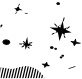
\includegraphics[width=\linewidth + 0.5cm]{neb/figures/stars.png}}
    \vspace{-0.7cm}\newline
    \boxtitle{SUMMARY}
    \vspace{-0.3cm}\newline
    {\bgroup
    \def\arraystretch{1.2}%
    \tiny
    \rowcolors{1}{white}{gray!8}
    \roboto
    \begin{tabular}{|m{0.15\linewidth}|m{0.15\linewidth}|m{0.15\linewidth}|m{0.15\linewidth}|m{0.15\linewidth}|}
    \BLOCK{for disposition1, disposition2, disposition3, disposition4, disposition5 in obstable}
        \hline
        \VAR{disposition1} & \VAR{disposition2} & \VAR{disposition3} & \VAR{disposition4} & \VAR{disposition5}\\
    \BLOCK{endfor}
    \hline
    \end{tabular}
    \egroup}

    \vspace{0.5cm}\newline
    \boxtitle{DMAG vs RMS}

    \mbox{\vspace{-0.3cm}\includegraphics[width=\linewidth]{neb/figures/dmag_rms.png}}

  } & \hspace{0.7cm}\parbox{\linewidth}{
    \boxtitle{LIGHT CURVES}
    \mbox{\hspace{-1cm}\includegraphics[width=\linewidth + 1cm]{neb/figures/suspects/lc0.png}}
  } \\
\end{tabular}
\newpage

\begin{tabular}{m{0.95\linewidth}m{0.05\linewidth}}
   \hspace{0.7cm}\parbox{\linewidth}{
    \boxtitle{LIGHT CURVES}
    \vspace{-0.45cm}\newline
    \mbox{\hspace{-0.5cm}\includegraphics[width=\linewidth + 0.8cm]{neb/figures/suspects/lcs1.png}}
  } & \parbox{\linewidth}{

  }
  \\
\end{tabular}

\newpage

\begin{tabular}{m{0.95\linewidth}m{0.05\linewidth}}
   \hspace{0.7cm}\parbox{\linewidth}{
    \boxtitle{LIGHT CURVES}
    \vspace{-0.45cm}\newline
    \mbox{\hspace{-0.5cm}\includegraphics[width=\linewidth + 0.8cm]{neb/figures/suspects/lcs2.png}}
  } & \parbox{\linewidth}{

  }
  \\
\end{tabular}
}
}